\subsection{\textbf{Histograma}}

De tal forma, dando continuidade ao assunto, o histograma é um método que auxilia na identificação de objetos e/ou características específicas da imagem, obtendo uma maior precisão nos resultados obtidos.

Segundo \citeonline{FILHO1999}, histograma são conjuntos de vários números no qual são indicados os percentuais de \textit{pixels} de uma imagem que possui determinados níveis de cinza. Estes valores, normalmente representados por gráficos, apresentam, para cada nível de cinza, o seu percentual de \textit{pixels} correspondente na imagem. Com base nessa análise feita pelo histograma, pode-se obter os níveis de contraste, brilho, e ate mesmo informações de predominância clara ou escura.

\begin{comment}
Para analisar cada elemento deste conjunto, \citeonline{FILHO1999} explicam, através de cálculos matemáticos, que é possível utilizando a equação a seguir:
\end{comment}

\citeonline{FILHO1999} explicam que, através de equações matemáticas, é possível obter um resultado satisfatório ao analisar cada elemento deste conjunto. Este trabalho não tem por finalidade apresentar e/ou explicar cálculos matemáticos que cada função executa.

%\begin{flalign*}
   P_r (r_k) = \frac{n_k}{n} \\
\end{flalign*}

onde:

\begin{math} 0 \le r_k \le 1 \end{math} \newline
k = 0, 1, ..., L-1, onde L é o número de níveis de cinza da imagem digitalizada; \newline
n = número total de \textit{pixels} na imagem; \newline
\begin{math} P_r (r_k) \end{math} = probabilidade do k-ésimo nível de cinza; \newline
\begin{math} n_k \end{math}= número de \textit{pixels} cujo nível de cinza corresponde a k.
 \newline

%Tabela comentada
\begin{comment}
Na tabela a seguir está sendo representado os exemplos matemáticos de histograma \cite{FILHO1999}.

\clearpage

\begin{table}[h]
\centering
\caption{{\footnotesize Exemplo de histograma.}}
\vspace{0.5cm}
\begin{tabular}{r|lr}
\hline
\hline 
Níveis de cinza (r_k) & n_k & p_r(r_k) \\ % Note a separação de col. e a quebra de linhas
\hline
\hline % para uma linha horizontal
0 & 1120    & 0,068 \\ 
1/7 & 3214  & 0,196 \\
2/7 & 4850  & 0,296 \\
3/7 & 3425  & 0,209 \\
4/7 & 1995  & 0,122 \\
5/7 & 784   & 0,048 \\
6/7 & 541   & 0,033 \\
1 & 455     & 0,028 \\  % não é preciso quebrar a última linha
\hline
\hline
Total: & 16384 & 1 \\
\hline
\hline
\end{tabular}
\end{table}
\\
\end{comment}

De forma a complementar o assunto, \citeonline{MAIZA2013} expressa em sua tese que, ao obter o histograma da imagem, pode-se alcançar medidas estatísticas dos níveis de cinza da imagem, como por exemplo o seu valor mínimo e máximo, valor médio, variância e desvio padrão. Portanto, o histograma seria como um método de probabilidade, onde o número de \textit{pixels} de um determinado nível de cinza pode ser utilizado para calcular um outro \textit{pixel} com o mesmo valor de cinza na imagem.

\begin{figure}[!htb]
\caption{ {\footnotesize Imagem (a) e seu respectivo histograma (b).}}
 
\centering % para centralizarmos a figura
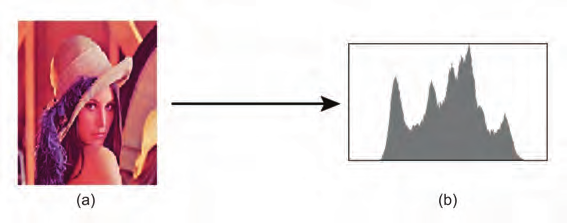
\includegraphics[width=11cm]{revisao-bibliografica/Figuras/Histograma.png}% leia abaixo
\label{figura:figura7}

\centering \subfloat {\footnotesize { Fonte: \cite{MAIZA2013} }}
{
\label{figura:figura7}
}
\end{figure}